% LaTeX file for resume 
% This file uses the resume document class (res.cls)

%\documentclass[margin]{res} 
\documentclass[10pt]{res}
\usepackage{graphicx}
\usepackage{wrapfig}
\usepackage{enumitem}
\graphicspath{ {/Users/haynes/Downloads/} }
\setlist{nosep,after=\vspace{0pt}}
%\topmargin=-0.4in
%\oddsidemargin -.25in
%\evensidemargin -.25in
%\textwidth=5.0in
%\textheight =10.4in
%\usepackage[margin=1.0in]{geometry}
\usepackage{multicol}
% the margin option causes section titles to appear to the left of body text 
%\textwidth=5.5in % increase textwidth to get smaller right margin
%\usepackage{helvetica} % uses helvetica postscript font (download helvetica.sty)
%\usepackage{newcent}   % uses new century schoolbook postscript font 
\tolerance=1
\emergencystretch=\maxdimen
\hyphenpenalty=10000
\hbadness=10000
\begin{document} 
 
\name{William Haynes Heaton, M.D., Ph.D.\\ [11pt]} % the \\[12pt] adds a blank line after name
 
%\address{  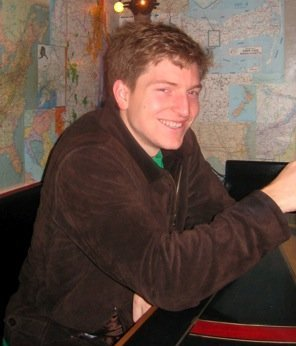
\includegraphics[scale=0.4]{pic} 1552 East Gate Way \#231 \\ Pleasanton CA, 94566 \\
  %      (256) 648-6432 \\ https://github.com/wheaton5 \\
    %    www.haynesheaton.com} 
%\begin{wrapfigure}{l}{0.25\textwidth}
%\centering
%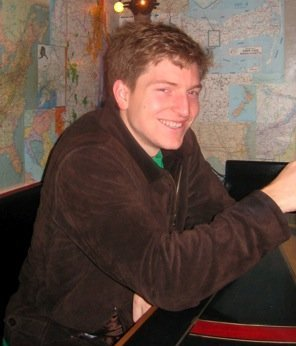
\includegraphics[scale=0.4]{pic}
%\end{wrapfigure}
\address{ 840 Dakota Dr \\ Auburn, AL 36832 \\
        (256) 648-6432  \\ https://github.com/wheaton5 \\
        www.haynesheaton.com}


 
\begin{resume} 
%\section{Education} 

%PhD (current) \hfill Sanger Institute, Cambridge University, Cambridge, UK \\
%MD May 2011 \hfill Brown Medical School, Providence, RI \\ 
%Computer Science May 2007 \hfill Brown University, Providence, RI 

%\newpage


\section{Education and Training}

	{\bf Cambridge University, Sanger Institute}
	\begin{itemize}[leftmargin=0.75in,topsep=2pt,noitemsep]
		\item[{\bf PhD}]  Computational Biology \hfill 2017-2021
		\begin{itemize}[label=$\bullet$, leftmargin=0.0in,noitemsep,topsep=-5pt]
			\item Advisors: Richard Durbin and Mara Lawniczak
			\item Projects:
				\begin{itemize}[noitemsep]
					\item Clustering mixed-sample scRNAseq data by genotype without a genotype reference.
					\item Haplotype resolved assembly via de novo phasing and long read haplotype binning.
					\item Pedigree assembly strategies.
				\end{itemize}
		\end{itemize}
	\end{itemize}
	{\bf Brown University}
	\begin{itemize}[leftmargin=0.75in,topsep=2pt, noitemsep]
		\item[{\bf MD}] Brown Medical School \hfill 2007-2011 
		\item[{\bf ScB}] Computer Science \hfill 2003-2007
			\begin{itemize}[label=$\bullet$, leftmargin=0.0in, noitemsep,topsep=-5pt]
				\item Advisor: Sorin Istrail
			\end{itemize}
	\end{itemize}
	\begin{itemize}[leftmargin=1.85in,topsep=5pt, noitemsep]
		\item[{\bf Student Researcher}] \hfill 2006-2007
			\begin{itemize}[label=$\bullet$, leftmargin=-1.1in, noitemsep,topsep=-5pt]
				\item Computer vision/ML to classify malignancy of histology images in bladder cancer.
			\end{itemize}
	\end{itemize}
	%{\bf Vanderbilt University}
	%\begin{itemize}[leftmargin=1.85in, topsep=2pt, noitemsep]
	%	\item[{\bf Visiting Researcher}] \hfill Summers 2005-2008
	%	\begin{itemize}[label=$\bullet$, leftmargin=-1.1in, noitemsep,topsep=-5pt]
	%			\item Advisor: Antonis Hatzopolous
	%			\item Project: BMP antagonist regulation of differentiation to cardiomyocyte lineages.
	%	\end{itemize}
	%\end{itemize}

%{\bf Student Researcher}, Brown University \hfill 2006 - 2007 
%\begin{itemize}
%\item Algorithmic Cancer Diagnosis. Computer vision techniques and machine learning to classify histology images of bladder cancer into normal, low malignancy, and high malignancy. (with Sorin Istrail, Professor of CS, Brown)
%\end{itemize}
%{\bf Visiting Researcher}, Vanderbilt University \hfill Summers 2005-2008 
%\begin{itemize}
%\item Researched Bone Morphogenic Protein antagonist regulation of differentiation of embryonic stem cells in to various cardiomyocyte lineages. Wet lab genetics including cell cultue, PCR, western blot, immunohistochemistry.
%\end{itemize}





\section{Papers}
\textbf{Haynes Heaton}, Arthur M Talman, Andrew Knights, Maria Imaz, Richard Durbin, Martin Hemberg, Mara Lawniczak. ``souporcell: Robust clustering of single cell RNAseq by genotype and ambient RNA inference without reference genotypes". \textbf{Nature Methods}. 2020. \\ \\
*\textbf{Most viewed paper in Genes 2019 -} \\
Sarah B Kingan*, \textbf{Haynes Heaton*}, Juliana Cudini, Christine C Lambert, Primo Baybayan, Brendan D Galvin, Richard Durbin, Jonas Korlach, Mara KN Lawniczak. ``A high-quality de novo genome assembly from a single mosquito using PacBio sequencing." \textbf{Genes}, 2019.
\\ \\
Virginia M Howick, Andrew JC Russell, Tallulah Andrews, \textbf{Haynes Heaton}, Adam J Reid, Kedar Natarajan, Hellen Butungi, Tom Metcalf, Lisa H Verzier, Julian C Rayner, Matthew Berriman, Jeremy K Herren, Oliver Billker, Martin Hemberg, Arthur M Talman, Mara KN Lawniczak. ``The Malaria Cell Atlas: Single parasite transcriptomes across the complete Plasmodium life cycle." \textbf{Science}, 2019.
\\ \\
Patrick Marks, Sarah Garcia, Alvaro Martinez Barrio, Kamila Belhocine, Jorge Bernate, Rajiv Bharadwaj, Keith Bjornson, Claudia Catalanotti, Josh Delaney, Adrian Fehr, Ian T Fiddes, Brendan Galvin, \textbf{Haynes Heaton}, et al. ``Resolving the full spectrum of human genome variation using Linked-Reads." \textbf{Genome Research}, 2019.
\\ \\
Mark JP Chaisson, Ashely Sanders, Xuefang Zhao, 19 authors, \textbf{Haynes Heaton}, 65 authors, Evan E Eichler, Charles Lee. ``Multi-platform discovery of haplotype-resolved structural variation in human genomes." \textbf{Nature Communications}, 2019.
\\ \\
Justin Zook, Jennifer McDaniel, Hemang Parikh, \textbf{Haynes Heaton}, Sean A Irvine, Len Trigg, Rebecca Truty, Cory Y McLean, Francisco M De La Vega, Marc Salit, Genome in a Bottle Consortium. ``An open resource for accurately benchmarking small variant and reference calls."  \textbf{Nature Biotechnology}, 2019.
\\ \\
Grace Zheng, Billy T. Lau, Michael Schnall-Levin, 17 authors,  \textbf{Haynes Heaton}, 34 authors, Serge Saxonov, Kevin D Ness, Benjamin J Hindson, Hanlee P Ji. ``Haplotyping germline and cancer genomes with high-throughput linked-read sequencing." \textbf{Nature Biotechnology} (2016).  
\\ \\
Vineeta Tanwar, Jeffery B. Bylund, Jianyong Hu, Jingbo Yan, Joel M. Walthall, Amrita Mukherjee, \textbf{William H. Heaton}, Wen-Der Wang, Franck Potet, Meena Rai, Sabina Kupershmidt, Ela W. Knapik, and Antonis K. Hatzopoulos. "Gremlin 2 promotes differentiation of embryonic stem cells to atrial fate by activation of the JNK signaling pathway." \textbf{Stem Cells}, 2014. 

\section{Patents}
Goldstein, Peter, \textbf{William Heaton}, Franco Preparata, and Eli Upfal. ``Distance maps using multiple alignment consensus construction." U.S. Patent Application 14/212,458, filed March 14, 2014. \\  \\
Kyriazopoulou-Panagiotopoulou, S., Marks, P., Schnall-Levin, M., Zheng, X., Jarosz, M., Saxonov, S., ... \& \textbf{Heaton, W. H.} (2016). U.S. Patent Application No. 15/019,928. 


\section{Invited talks}
Haynes Heaton. ``New approaches to generate single insect haplotype assemblies." Plant and Animal Genomes conference 2020. \\ \\ 
Haynes Heaton. ``De Novo phasing: toward haploid assemblies from diploid organisms without a trio." Darwin Tree of Life consortium workshop. 2019. \\ \\
Haynes Heaton. ``Novel genetic variation and validation using Linked Reads." Genome in a bottle consortium workshop. 2016.

\section{Poster presentations}
Haynes Heaton. ``Alignment and Variant Calling in Segmental Duplications with Linked-Read Data". Genome Informatics. 


\section{Teaching}
{\bf Head Teaching Assistant} Computational Molecular Biology \hfill Fall 2006, 2007 \\
{\bf Teaching Assistant} Introduction to Computer Systems \hfill Fall 2005 \\ 
{\bf Head Teaching Assistant} Introduction to Scientific Computing \hfill Spring 2005, 2006 \\
{\bf Teaching Assistant} Introduction to Scientific Computing \hfill  Spring 2004 \\

\section{Industry \\Experience}

{\bf Senior Scientist}, 10X Genomics \hfill 2014-2017 \\
Algorithm and software development on genomics platform bringing long range genetic information to nextgen short-read sequencing. We use a microfluidic system to attach the same barcode to every read originating from a long DNA molecule while different molecules get different barcodes with high probability. 
\begin{itemize}
\item Developed new linked-read aligner ``Lariat" which takes into account the molecule information when finding its mapping. This produces fewer mismapped reads and is able to map into many repeat regions of the genome with high confidence. (lead on this project)
\item Invented novel phasing probabilistic model which is able to filter variants that do not haplotype consistent. 
\item Head of short variant calling and data analysis, metrics, ground truth analysis of short variants.
\item Created a system of haploid variant calling to improve sensitivity. 
\item Worked with biochemists and chemists to create data metrics that allow them to continuously improve the data quality.
\end{itemize}


{\bf Senior Software Engineer: Scientific Computing}, GNS Healthcare, Cambridge MA \hfill 2013 - 2014 \\
Part of a team working on causal bayesian network machine learning with MCMC to sample graph structure of the bayesian nets. \\
\begin{itemize}
\item Contributed to methods in post learning simulation, analysis, and clustering.
\item Developed and supported Amazon EC2 execution of our platform using Starcluster.
\item Created distribution process for our post learning simulation using Hadoop on Amazon Elastic map reduce. 
\end{itemize}


{\bf Computational Scientist,} Nabsys, Providence RI \hfill 2011 - 2013 \\
Developed algorithms for a nano channel DNA mapping startup. Collaborated with Biochemistry and Electrical Engineering teams as well as consulting CS professors to make novel methods addressing data produced by a unique assay -- long (10s-100s of kilobases) DNA fragments with tag molecules attached to sequence specific sites are run through a solid-state nano-detector, creating data analogous to ordered restriction maps (or bionano genomics data). \\

\begin{itemize} %\itemsep -2pt  % reduce space between items
\item Developed genetic distance map de novo assembly software with computational biologist Peter Goldstein. 
\item Created novel multiple alignment using a probabilistic, graph theoretic approach. This allowed us to reduce error through averaging distances and consensus voting over multiple measurements. (Lead on this project. Patented, with Peter Goldstein, Computational Biologist Nabsys)
\item Wrote signal processing software employing standard EE methods as well as HMMs and watershed algorithm for feature extraction. Created interactive data visualization package. (Lead on this project managing two employees.)
\end{itemize}

\section{Software Engineering}
{\bf Languages}
\begin{tabular}{l l}
{\bf Expert} & {\bf Proficient} \\
Rust, Python, R, Go, Java & C/C++, Javascript (D3.js), Matlab/Octave \\
\end{tabular}

\section{Techniques and skills}
\emph{Machine Learning} - linear/logistic with various regularizers, SVMs/SVRs with kernels, neural nets (DNN, CNN, RNN, deep autoencoders etc), causal Bayesian nets, decision/regression trees/random forrest, Gaussian Processes, tensorflow \\
\emph{Dimensionality Reduction} - PCA, SVD, random projections/sparse random projections, tSNE, deep autoencoders \\
\emph{Clustering} - K-means, hierarchical, K-nearest neighbors, mixture of gaussians, graph clustering (spectral, markov clustering), fuzzy c-means, GMMs / other mixture models including sparse mixture models. \\
\emph{Temporal/Series Pattern Recognition} - HMMs (viterbi, forward/backward, Baum-Welch), Fourier transform
\emph{Combinatorial optimization} - Metropolis Hastings, MCMC, simulated annealing, dynamic programming, branch and bound
\emph{Statistical inference} - variational inference, MCMC with STAN, tensorflow probability, edward
\end{resume} 
\end{document} 


